\section{Analyse}
\label{sec:sha256:analyse}

In dieser Analyse geht es um eine oberflächliche Betrachtung der Rundenfunktion und des vollständigen Algorithmus.
Ziel ist es ein Verständnis dafür zu entwickeln, was eine Umkehrung der Berechnung verhindert und welche Berechnungen
notwendig wären, um bestimmte Ziele zu erreichen.

\subsection{Rundenfunktion}
In Abbildung \ref{fig:sha256coreA} ist noch einmal die Rundenfunktion mit einigen Markierungen dargestellt.
Bei dem Versuch, die Funktion umzukehren, ist sofort ersichtlich, dass A bis C und E bis G direkt übernommen werden können.

\begin{figure}[!h]
  \centering
  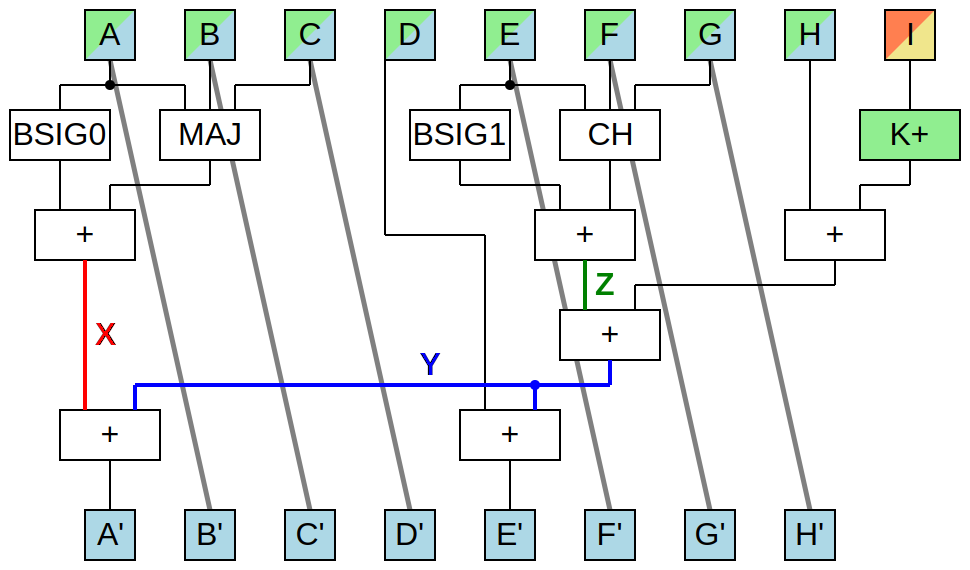
\includegraphics[scale=0.4]{images/sha256coreA}
  \caption{Analyse einer SHA256-Runde}
  \label{fig:sha256coreA}
\end{figure}

Dadurch lassen sich auch \textcolor{red}{\textbf{X}} und \textcolor{Strong Green}{\textbf{Z}} direkt berechnen.
Mit Hilfe von \textcolor{red}{\textbf{X}} lässt sich schließlich \textcolor{blue}{\textbf{Y}} berechnen, was zu D führt.
Formell ist dieser Zusammenhang in Abbildung \ref{eq:calcD} dargestellt.

\begin{figure}[!h]
  \begin{tabbing}
    XXXXXXXXXXXXXXXXXXXXX\=XX\=XX\=XXXXXX\=XXXX\=XX\=XX\=XXXXXXXX \kill
    \>A'\>=\>\textcolor{red}{\textbf{X}} + \textcolor{blue}{\textbf{Y}}\>$\Rightarrow$\>\textcolor{blue}{\textbf{Y}}\>=\>A' - \textcolor{red}{\textbf{X}}\\
    \>E'\>=\>D + \textcolor{blue}{\textbf{Y}}\>$\Rightarrow$\>\textcolor{blue}{\textbf{Y}}\>=\>E' - D\\
    \>~\\
    \>\>\>E' - D\>=\>A' - \textcolor{red}{\textbf{X}}\\
    \>\>\>-D    \>=\>A' - \textcolor{red}{\textbf{X}} - E'\\
    \>\>\>D     \>=\>\textcolor{red}{\textbf{X}} + E' - A'
  \end{tabbing}
  \caption{Berechnung von D}
  \label{eq:calcD}
\end{figure}

\subsection{Angriffsvektoren}

A bis H bei gegebenem Hash und Eingabe berechnen.\\
I jeweils bekannt jedoch fehlt A' bis H' da durch Addition mit Geheimnis "`maskiert"'.\\
Würde einen Angriff auf das Lösen einer einmalige Anwendung der 64 Runden bei beliebigen Eingabelängen reduzieren.
~\\
Eingabe bei gegebenem A bis H und Hash berechnen.\\
Problem ist es H/I zu bestimmen wie im Abschnitt vorher beschrieben\\
~\\
Geburtstagsparadoxon ausnutzen, ausgabe gleichsetzen und unterschied bei eingabe fordern